\documentclass[tikz,border=8pt]{standalone}
\usepackage{pgfplots}
\pgfplotsset{compat=1.18}
\begin{document}
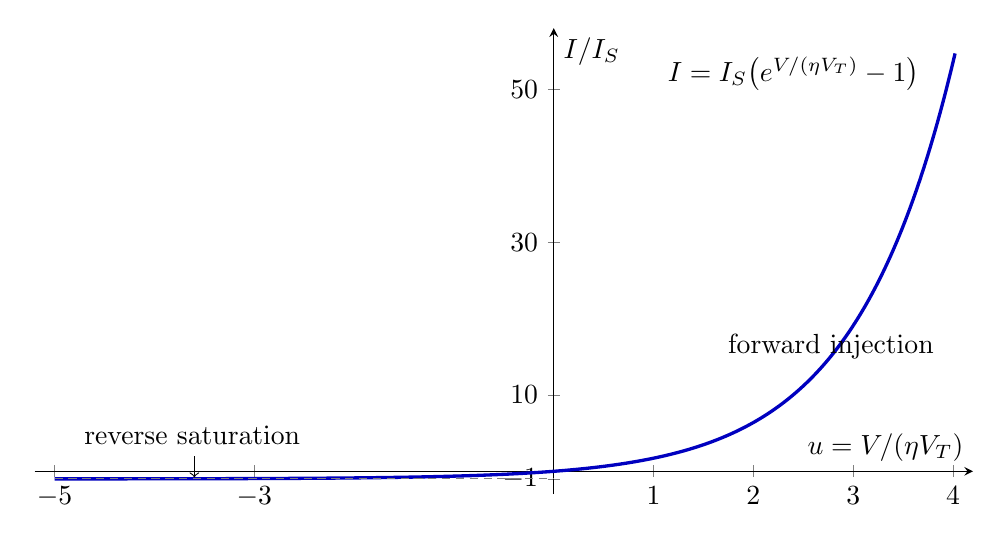
\begin{tikzpicture}
\begin{axis}[
  width=13.5cm,height=7.5cm,
  xmin=-5.2,xmax=4.2,ymin=-3.0,ymax=58,
  axis lines=middle,
  xlabel={$u=V/(\eta V_T)$},ylabel={$I/I_S$},
  xtick={-5,-3,0,1,2,3,4},ytick={-1,0,10,30,50},
  clip=false
]
\addplot[very thick,blue!75!black,domain=-5:4.02,samples=360]{exp(x)-1};
\draw[densely dashed,gray] (axis cs:-5,-1)--(axis cs:0,-1);
\node[anchor=south east,fill=white,inner sep=2pt] at (axis cs:3.72,49)
  {$I=I_S\!\left(e^{V/(\eta V_T)}-1\right)$};
\node[anchor=south west] at (axis cs:-4.8,2.2) {reverse saturation};
\draw[->] (axis cs:-3.6,2.0)--(axis cs:-3.6,-0.8);
\node[anchor=south west] at (axis cs:1.65,13.5) {forward injection};
\end{axis}
\end{tikzpicture}
\end{document}
